\begin{figure}
    \centering
    \begin{subfigure}{0.48\linewidth}
        \centering
        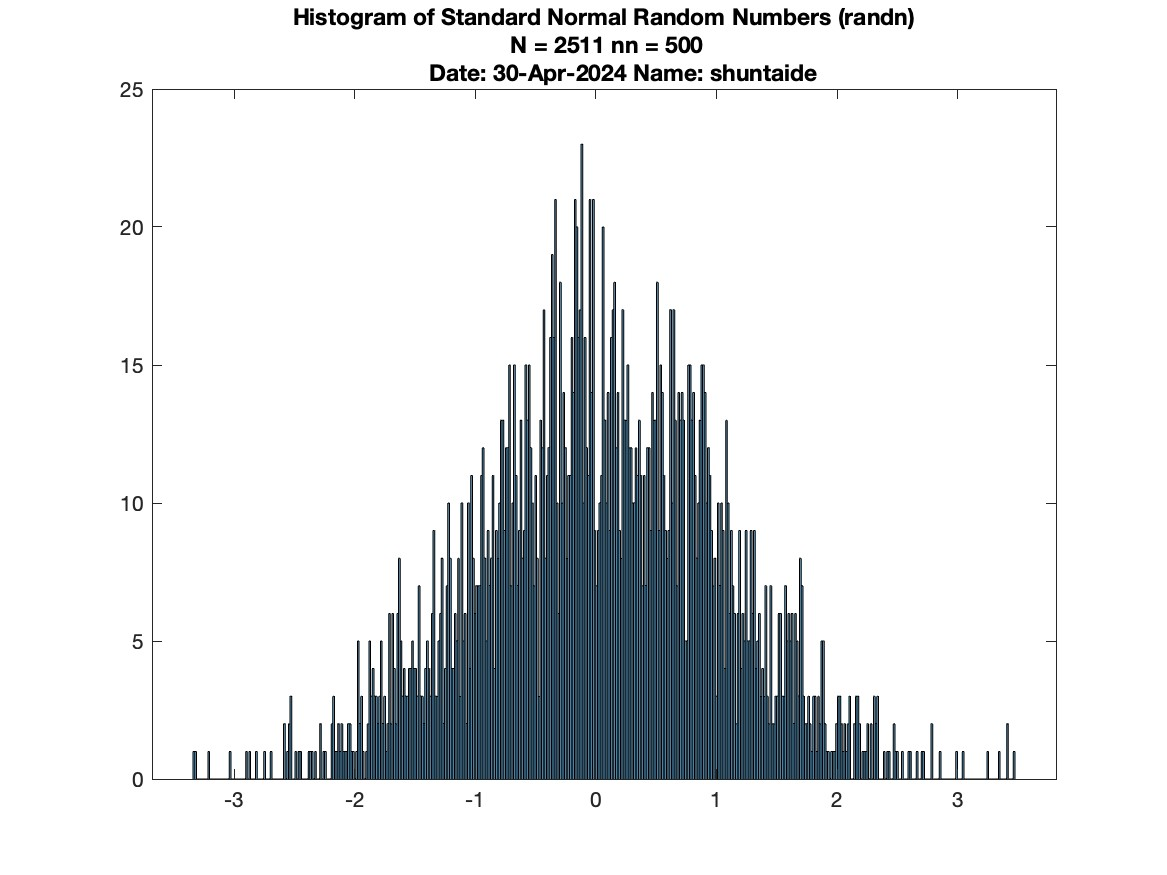
\includegraphics[width=0.8\textwidth]{src/figures/standard-normal/randn_hist_N=2511_nn=500.jpg}
        \subcaption{$N=2511$, $nn=500$}
    \end{subfigure}
    \begin{subfigure}{0.48\linewidth}
        \centering
        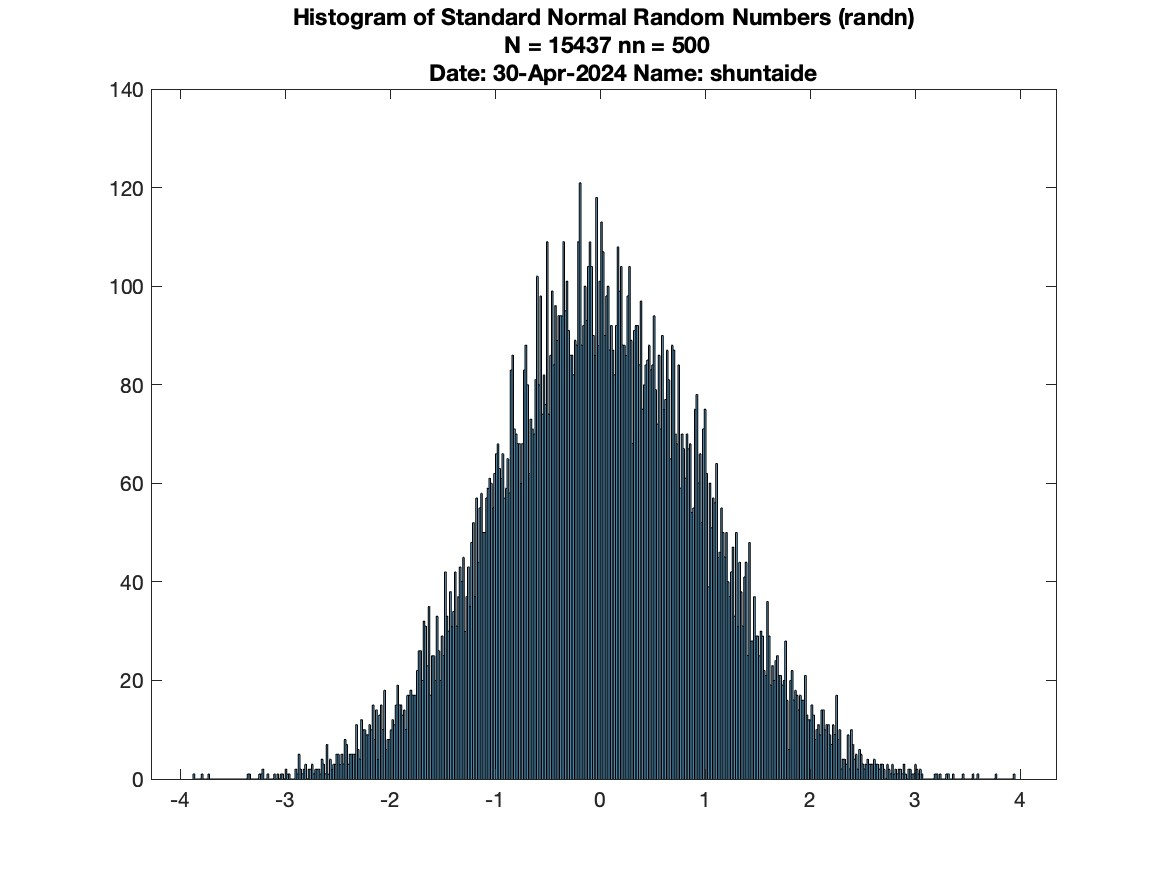
\includegraphics[width=0.8\textwidth]{src/figures/standard-normal/randn_hist_N=15437_nn=500.jpg}
        \subcaption{$N=15437$, $nn=500$}
    \end{subfigure}
    \begin{subfigure}{0.48\linewidth}
        \centering
        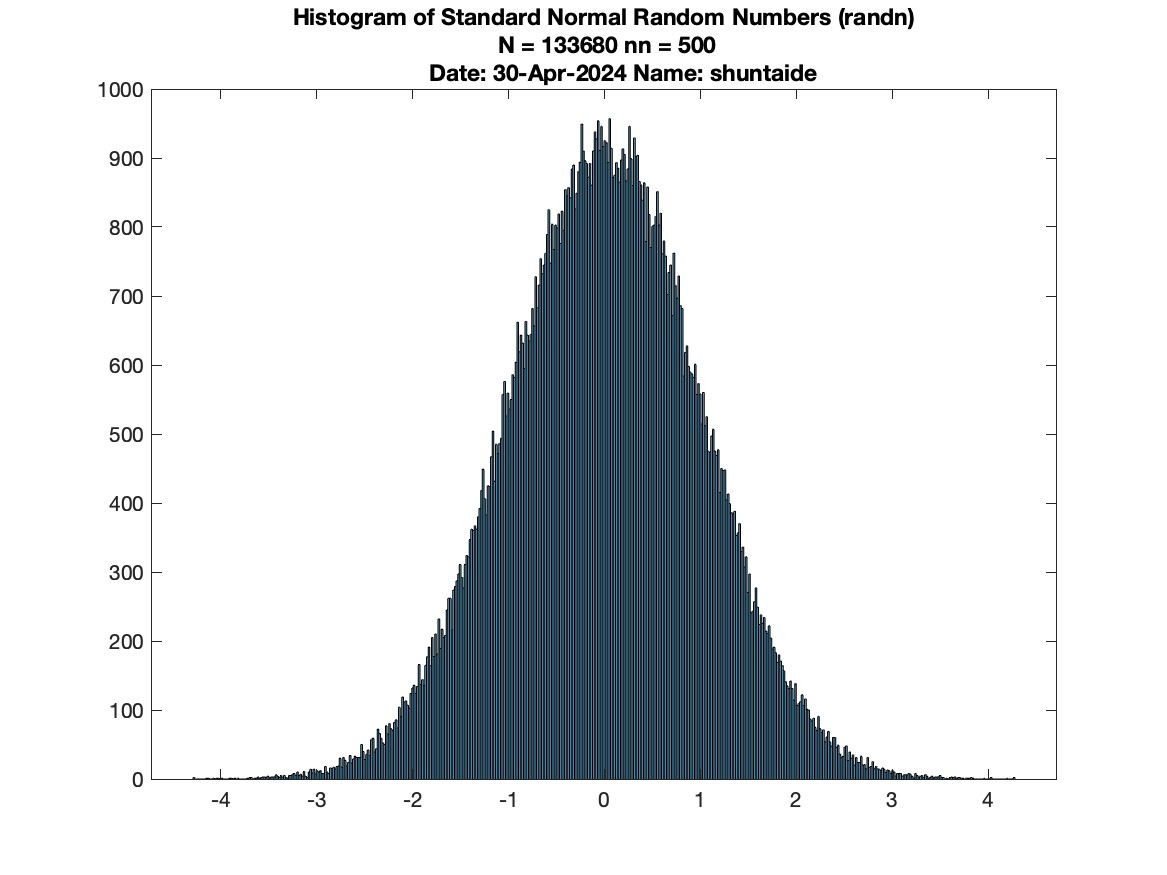
\includegraphics[width=0.8\textwidth]{src/figures/standard-normal/randn_hist_N=133680_nn=500.jpg}
        \subcaption{$N=133680$, $nn=500$}
    \end{subfigure}
    \begin{subfigure}{0.48\linewidth}
        \centering
        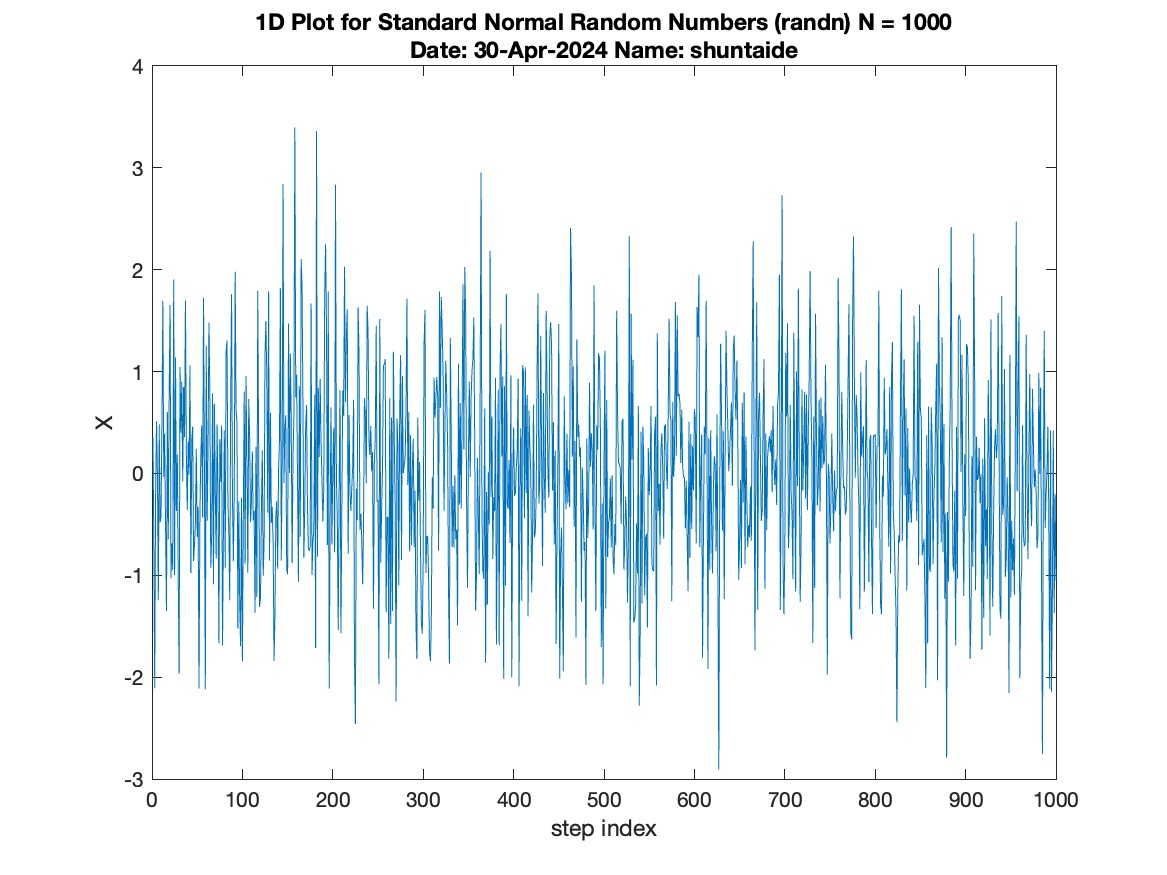
\includegraphics[width=0.8\textwidth]{src/figures/standard-normal/randn_1Dpl_N=1000.jpg}
        \subcaption{生成回と値の関係}\label{fig:standard-normal-1Dpl}
    \end{subfigure}
    \begin{subfigure}{0.48\linewidth}
        \centering
        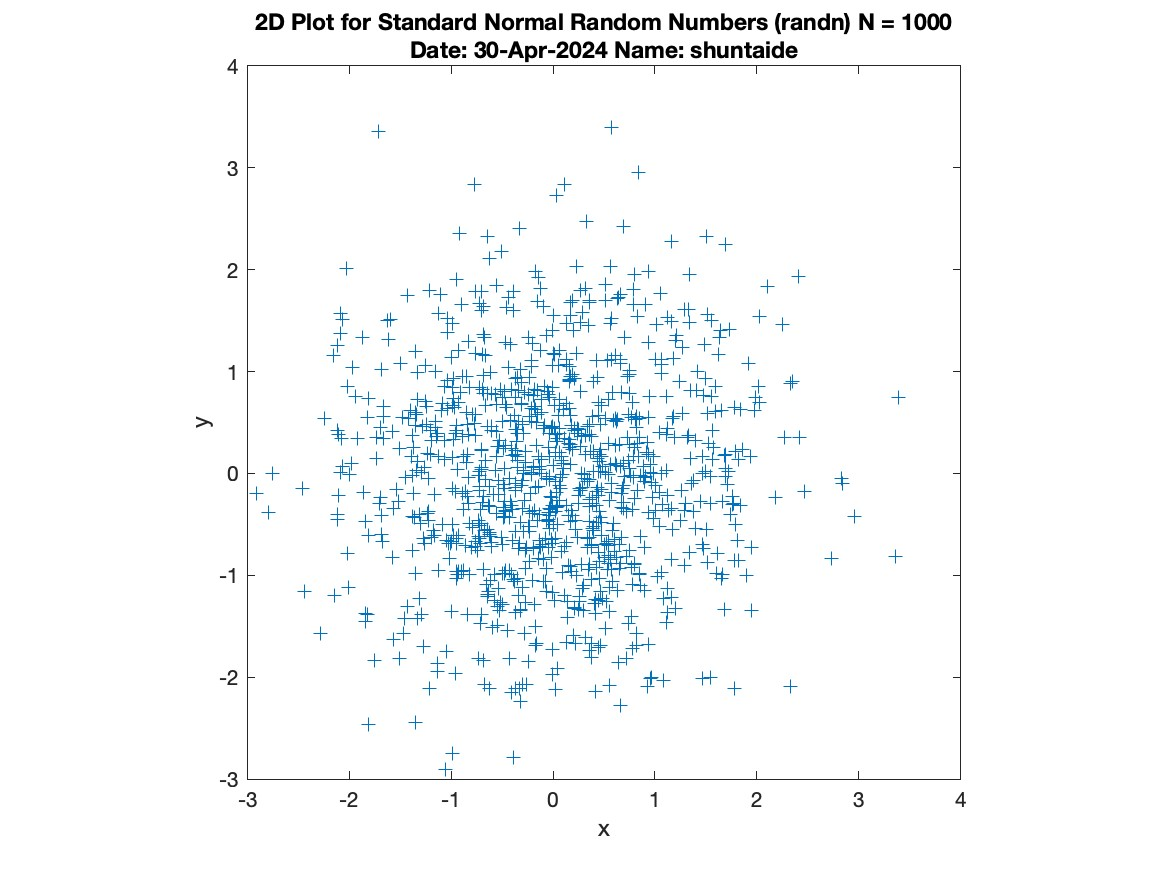
\includegraphics[width=0.8\textwidth]{src/figures/standard-normal/randn_2Dpl_N=1000.jpg}
        \subcaption{横軸が奇数回に生成された値、縦軸が偶数回に生成された値}\label{fig:standard-normal-2Dpl}
    \end{subfigure}
    \begin{subfigure}{0.48\linewidth}
        \centering
        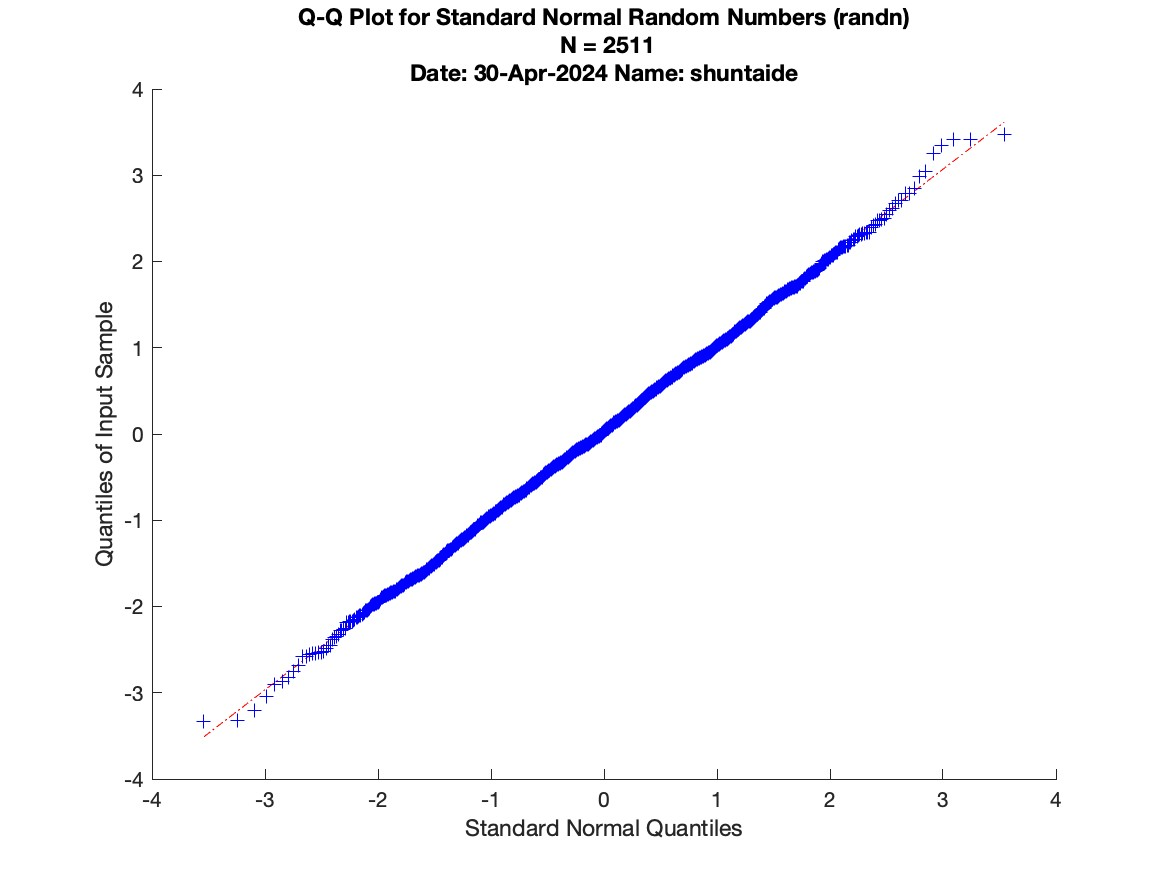
\includegraphics[width=0.8\linewidth]{src/figures/standard-normal/randn_qqpl_N=2511.jpg}
        \subcaption{QQプロット($N=2511$)}\label{fig:standard-normal-qqpl-2511}
    \end{subfigure}
    \begin{subfigure}{0.48\linewidth}
        \centering
        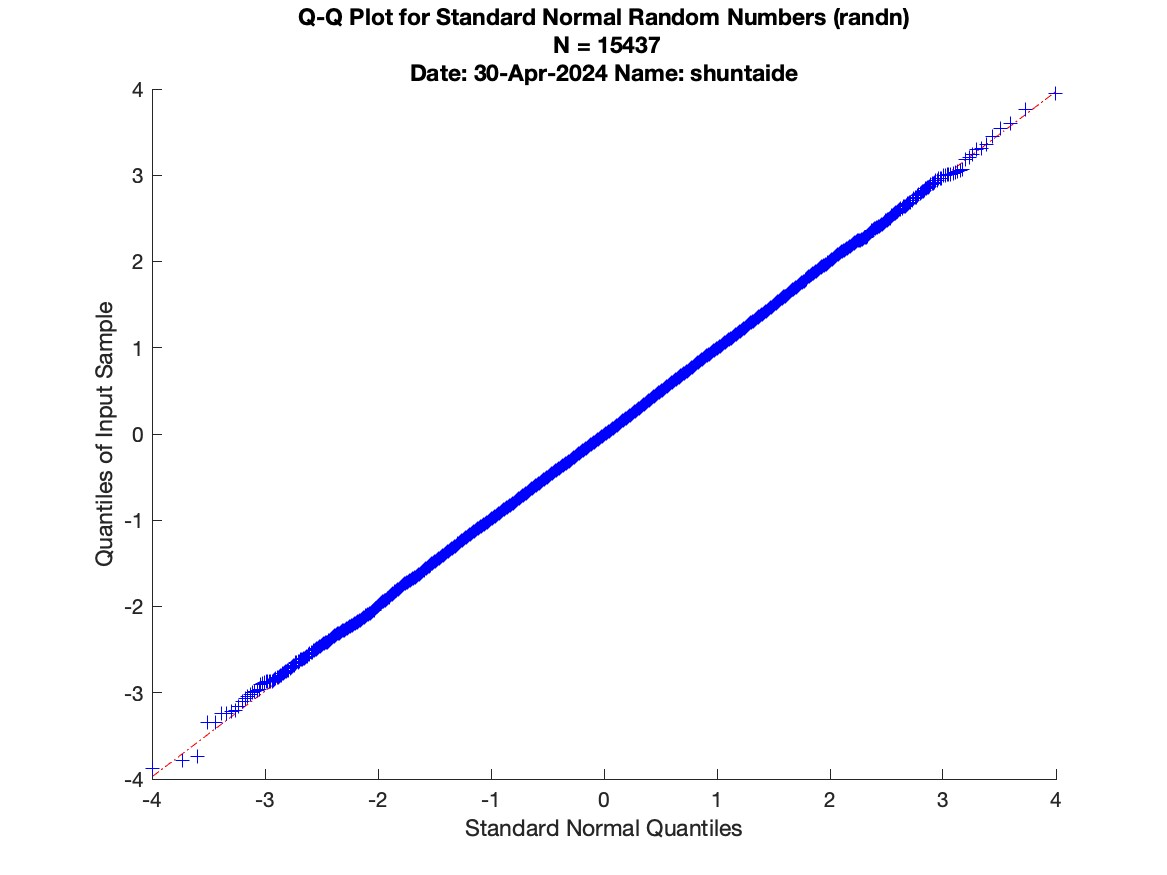
\includegraphics[width=0.8\linewidth]{src/figures/standard-normal/randn_qqpl_N=15437.jpg}
        \subcaption{QQプロット($N=15437$)}\label{fig:standard-normal-qqpl-15437}
    \end{subfigure}
    \begin{subfigure}{0.48\linewidth}
        \centering
        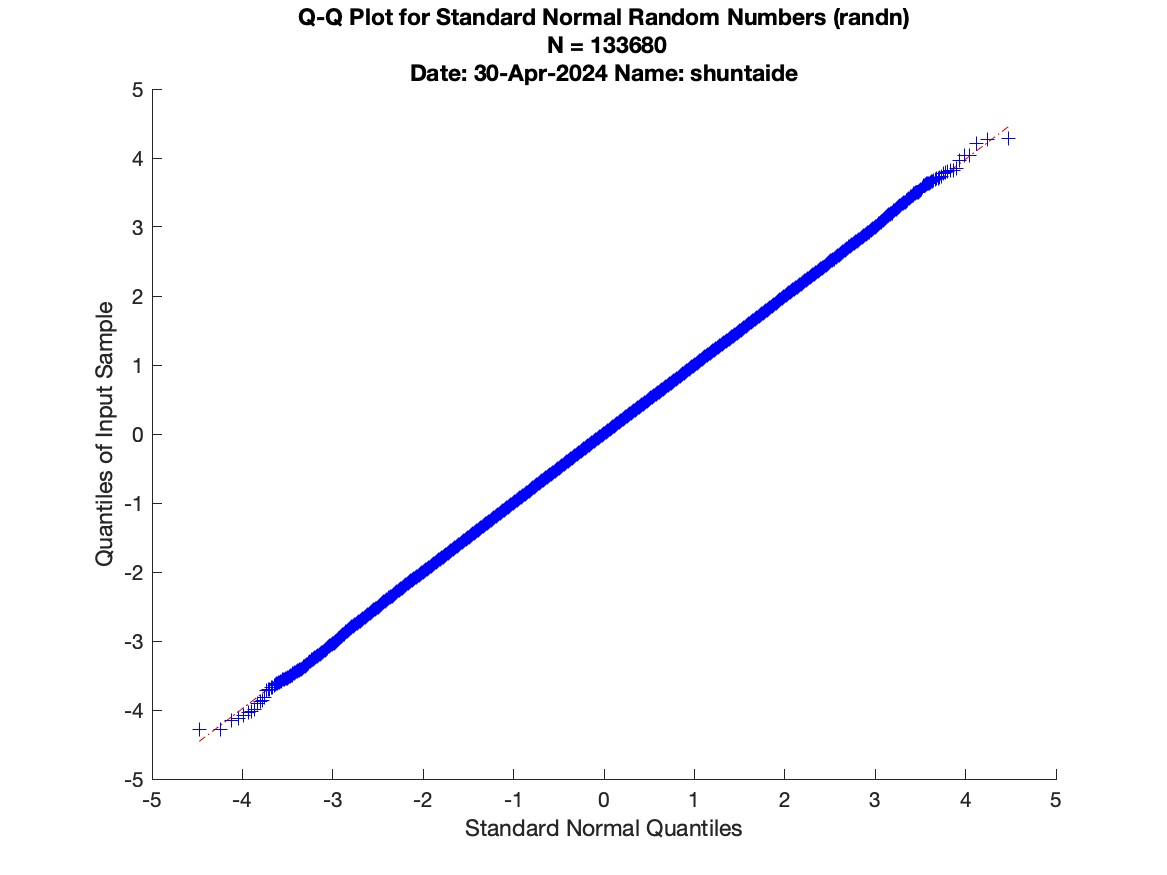
\includegraphics[width=0.8\linewidth]{src/figures/standard-normal/randn_qqpl_N=133680.jpg}
        \subcaption{QQプロット($N=133680$)}\label{fig:standard-normal-qqpl-133680}
    \end{subfigure}
    \caption{標準正規乱数の生成結果}\label{fig:standard-normal-random}
\end{figure}
